%-------------------------------------------------------------------------------
% Definitions
%-------------------------------------------------------------------------------
% here we define authors and titles
%
\providecommand{\theauthorsfull}{Anton Biryukov, Jan Dettmer and David Eaton} %full list of authors - eg Mirko van der Baan and David Eaton
\providecommand{\theauthorsshort}{Biryukov et al.} %short list of authors (max 40 characters} - eg Van der Baan and Eaton or Van der Baan et al.
\providecommand{\thetitlefull}{Event origin depth uncertainty - steps towards estimation and mitigation using waveform similarity}
\providecommand{\thetitleshort}{Location depth error mitigation} % max 40 characters
%-------------------------------------------------------------------------------
% REPORT SECTION
%-------------------------------------------------------------------------------

%\chapter[\theauthorsshort: \thetitlefull]{\thetitlefull \\ \vbox{}
%\vbox{}
%{\small\em 
% place address here
%${}^a$ Department of Geoscience, University of Calgary, Calgary, AB, T2N 1N4, Canada.  E: anton.biryukov@ucalgary.ca \\[-10pt]
%}} % don't remove!
%

\chapter[\theauthorsshort: \thetitlefull]{\thetitlefull \\ \vbox{}
{\LARGE\em  Anton Biryukov, Jan Dettmer and David Eaton}\\ %Replace with your own list of authors
\vbox{}
{\small\em 
% place address here
${}^a$ Department of Geoscience, University of Calgary, Calgary, AB, T2N 1N4, Canada.  E: anton.biryukov@ucalgary.ca \\[-10pt]
%${}^b$ Dept. of Physics, Univ. of Alberta, Edmonton, AB, T6G 2G7, Canada.  E: Mirko.vanderBaan@ualberta.ca
}} % don't remove!



\rhead[Microseismic Industry Consortium Vol. \thereportvolume\ -- Chapter \thechapter]{\em \thetitleshort}
\lhead[\theauthorsshort]{Microseismic Industry Consortium Vol. \thereportvolume\ -- Chapter \thechapter}

%
\section*{Summary}
%
The induced seismicity event localization using inverse kinematic algorithms is still a problem requiring special attention. Often a catalog of events detected and located using limited on-surface instrumentation lacks the precision of origin depth. Such errors can hinder the interpretation of activated zones using seismicity as a proxy.

On one hand, the location constraints are affected by the inaccuracy of the velocity model, limited acquisition geometry and the assumptions inherited by the location algorithm. The issue becomes even more aggravated when only surface arrays are employed, where the geometry strongly favors the accuracy of epicentral location as opposed to depth location. The reported uncertainty of the depth location is sometimes comparable to a formation thickness or even the origin depth itself.

Finding additional features of the seismic signal that could be informative of its origin can be a first step towards constraining the depth uncertainty. Therefore, the purpose of this study was two-fold. First, we characterized the uncertainty in the event origin due to the error in the effective velocity model used in event location. Using Monte-Carlo simulations for a given velocity model uncertainty, the event origin and the receiver array we simulate the traveltimes at the stations and then relocate the event using the baseline velocity model. We show that the presence of a low velocity zone (LVZ) can cause the non-uniqueness and a spread of the solution over a large depth range. This spread was found to depend on the scale of the velocity model uncertainty, whereas the epicenter of the event showed higher stability with respect to velocity model perturbations. Subsequently, a wave number integration method is utilized to simulate the synthetic seismograms from the synthetic earthquakes spanning the depth range of 2-5km, covering LVZ. For a fixed focal mechanism and frequency content, we numerically generate a bank of waveforms corresponding to the virtual events with known locations. The bank is then divided into a training, cross-validation and test parts. A set of classifiers is trained to predict the event location with respect to LVZ based on arrival times and statistical features of the signal waveforms. We demonstrate that adding several features of the signal, descriptive of its origin can improve the location depth constraint, as opposed to using arrival times only as predictor variables.
%
\section{Introduction}
%

\section{Methods}
%
This section provides a brief overview of the methods employed in this study. As our first goal was to estimate of the uncertainty in origin depth, we start with a brief description of the travel time calculation method based on the ray theory, followed by the summary of the event location algorithm employing the predicted travel times. Our second goal was to implement a classifier capable of determining the origin signal based on the arrival times and signal features. Therefore, this section also provides the work flow for preparing the feature set from the event waveforms and training such a classifier on the available data.

\section{Generalized workflow}
This report is particularly focused on estimating the depth error due to the velocity model uncertainty. That is, we want to evaluate the jitter in the hypocenter location due to inaccuracy in the approximation of the true velocity model as a 1D layered cake model derived from $V_{p}$ and $V_{s}$ logs. Specifically, we would like to simulate the travel times from many virtual events with a fixed origin but variable velocity model. These trave ltimes are then used for relocating the events, that should potentially result in a cloud centered at the origin. The spatial dimensions and the shape of the cloud can give a quantitative insight into how sufficient the 1D velocity model assumption might be for a particular region and acquisition geometry.

Therefore, the general workflow can be summarized in several key steps as follows:
\begin{itemize}
 \item determine the background (expected) velocity model from the sonic logs,
 \item carry out many (9000) Monte-Carlo (MC) simulations for the travel time sets in a perturbed velocity model for an event with a fixed origin,
 \item treating each travel times set independently, locate the event corresponding to the set using background velocity model,
 \item analyze the PDF of the obtained distribution.
\end{itemize}



\subsection{Monte - Carlo travel time simulations}
 As no anisotropy or 2D elastic profile information was available, the baseline velocity model was approximated as a 1D laterally homogeneous layered medium. The elastic parameters for the layers were derived from the sonic wellbore logs. The velocity uncertainty in this study is modeled through applying a random normal perturbation of $V_{p}$ and $V_{s}$ within a layer, while keeping the thickness of the layers constant. The standard deviation of the perturbation is a fraction of the velocity value within the layer. An example of the velocity profile distribution with the 6\% standard deviation is shown in Figure \ref{fig:vpvs}, with color showing the probability density function for the values of $V_{p}$ and $V_{s}$ within the layer.

\begin{figure}[htb]
\begin{center}
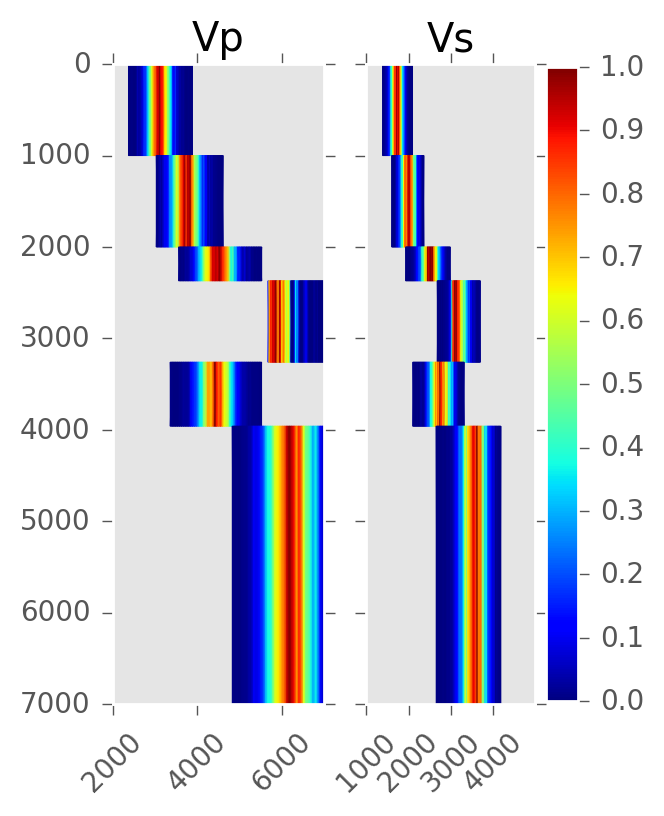
\includegraphics[width=0.7\linewidth,angle=0]{./AntonBiryukov_bibtex/VpVs.png}
\end{center}
\vspace{-4mm}
\caption{An example of the distribution of velocity profile used in the Monte-Carlo simulations. The color represents the values of probability density function of the velocity distribution. Note the limited variation of the layer above LVZ due to the creation of the shadow zone.}
\label{fig:vpvs}
\end{figure}

Currently, there exist various methods for computing synthetic seismograms (\citet{kennett_seismic_2001}, \citet{chapman_fundamentals_2004}). In the case of a 1D layered medium the classic seismic ray theory can produce an exact solution for the phase travel times assuming high frequency content of the signal, at a very low computational cost. Therefore, a Python-based implementation of a ray tracing method (Pyrocko-Cake by S. Heimann, available at http://emolch.github.io/pyrocko/) was chosen as a best fit-for-purpose method. Pyrocko-Cake allows robust obtaining travel times for a custom phase (e.g. direct P ($t_{p}$) and a direct S ($t_{s}$)) between a source and a receiver specified.


It is important to notice that for some of the MC realizations the travel times for all four stations were not available due to the strong velocity contrast created at 3200 meter depth. The presence of the contrast caused significant reflection leading to shadowing of the direct P-phase at larger offsets, and as such the realizations  discarded from the analysis. That effect is visible in the Figure \ref{fig:vpvs} by a limited accepted variation of $V_{p}$ within the layer at 2500 - 3200 meters depth.

\subsection{Event origin location} % Mention somewhere in discussion / intro the comparison between Linearized and DIRECT SEARCH!!!!!!!!!!!!!!!!!!!!!
In the case of the limited recording geometry and a velocity model with sharp horizontal interfaces, a probabilistic direct global-search procedure was shown to outperform the linearized location methods and adequately determine the complete location PDF of the event, converging to a global maximum (\citet{lomax_earthquakeearthquake_2009}). Therefore, we opted for employing the probabilistic, non-Linear, global-search earthquake location algorithm implemented in the NonLinLoc software \cite{lomax_precise_2001}. NonLinLoc has gained its popularity due to simple logic and easy-to-use interface, its robustness and currently is transitioning to become a standard for regional and global earthquake location.

The NonLinLoc program outputs a misfit function, an estimate of the posterior PDF for the spatial hypocenter location, and other results using stochastic, Metropolis-Gibbs sampling approach. The errors in the phase time picks and in the forward problem (travel-time calculation) are assumed to be Gaussian. This assumption allows for the analytic calculation of a maximum likelihood origin time given the observed arrival times and the calculated travel times between the observing stations and a point in space. To achieve efficiency for complicated, 3D models, the travel-times between each station and all nodes of the spatial grid are calculated once and then stored on disk as travel-time grid files.

The algorithm searches the grids to find the best-fitting set of travel-times that would approximate the observed travel times for an event. In this simulations we use only local four stations, and utilize both P and S picks for each station, a total of 8 travel times. The x,y,z volume used for grid-search or Metropolis-Gibbs location must be fully contained within the 3D travel-time grids. This limits the largest station distance that can be used for location since the 3D travel-time computation and the size of the output time-grid files grow rapidly with grid dimension. In our case however, the zone of interest is well constrained within the station array, thus the zone of search satisfy the NonLinLoc requirements.

\subsection{Synthetic waveform modeling}
The synthetic waveforms used for event origin classification were produced using the wavenumber integration method implemented in CPS suite (\cite{herrmann_computer_2013}). For the particular case of 1D layered homogeneous media, CPS allows one to obtain the full waveforms from the source much quicker than 2D Finite Difference methods commonly used for similar purposes.

For each of the source-receiver pairs simulated in the model we generate a database of Green's functions. The Green's functions are then convolved with the source wavelet of the given dominant frequency $f=2.5$ Hz and a given moment tensor $M_{i,j}$ corresponding to a pure explosive source (identity matrix). To achieve variability in the signal waveforms and mimic realistic amplitude uncertainty, the moment tensor was perturbed with a Gaussian noise:
\begin{equation}
 M_{i,j} = 1 + \sigma_{m},
\end{equation}
where $\sigma_{m} = 0.1$ is the standard deviation of the perturbation. The uncertainty of the velocity model is taken into account by applying a random shift in time to the waveforms, and perturbing $t_{p},t_{s}$ with the standard deviation derived from the Monte-Carlo simulations described above. Subsequently, a set of statistical and deterministic features is extracted from the waveforms in order to bring more information about the origin of the signal. Specifically, we want to describe the signal properties that are expected to change due to the relative position of the origin with respect to the strong reflector. Prior to the feature extraction, the signals are all normalized to a unit amplitude. We then obtained the envelope of the signal on the vertical channel using Hilbert transform and chose the following features as the proxy:
\begin{itemize}
 \item kurtosis of the signal envelope - to show the peaked-ness of the signal and discern between signals with strong and weak multiple reflections,
 \item mean value of the envelope,
 \item standard deviation of the envelope - to show the variability in the envelope,
 \item area under the envelope,
 \item the ratio of the signal energy contained between $t_{p}$ and $t_{s}$ with respect to the whole trace
 \item number of zero-crossings of the envelope derivative - to count the number of local extrema of the envelope
\end{itemize}

The procedure of modeling and feature extraction is then repeated over the set of values for the moment tensor $M_{i,j}$ and locations covering the range of 2000-5000 meters, thus creating an exhaustive dataset for the subsequent classification. It is important to notice that the list of features is by no means exhaustive and can be altered and augmented if necessary. The choice of the most representative features for the particular problem is a complicated task by itself and is therefore out of scope for this study. Our main goal was to show whether adding easily available information can positively affect the location accuracy judged by the classification score or not.
\subsection{Signal classification}
The signal database obtained from the synthetic waveform modeling procedure has been divided into 3 classes by the origin depth of the event: (i) above LVZ, (ii) within LVZ, and (iii) below LVZ. The database was then split into the training (70\% of the total data) and the test datasets (30\% of the total). For each item in the dataset we have obtained a set of features and its class.

A set of classification algorithms is then trained on the training data in order to predict the focal depth of the event (its class) given a set of features of an event of interest from the test data. The concept is briefly illustrated in the Figure \ref{fig:classes}.

\begin{figure*}[htb]
\begin{center}
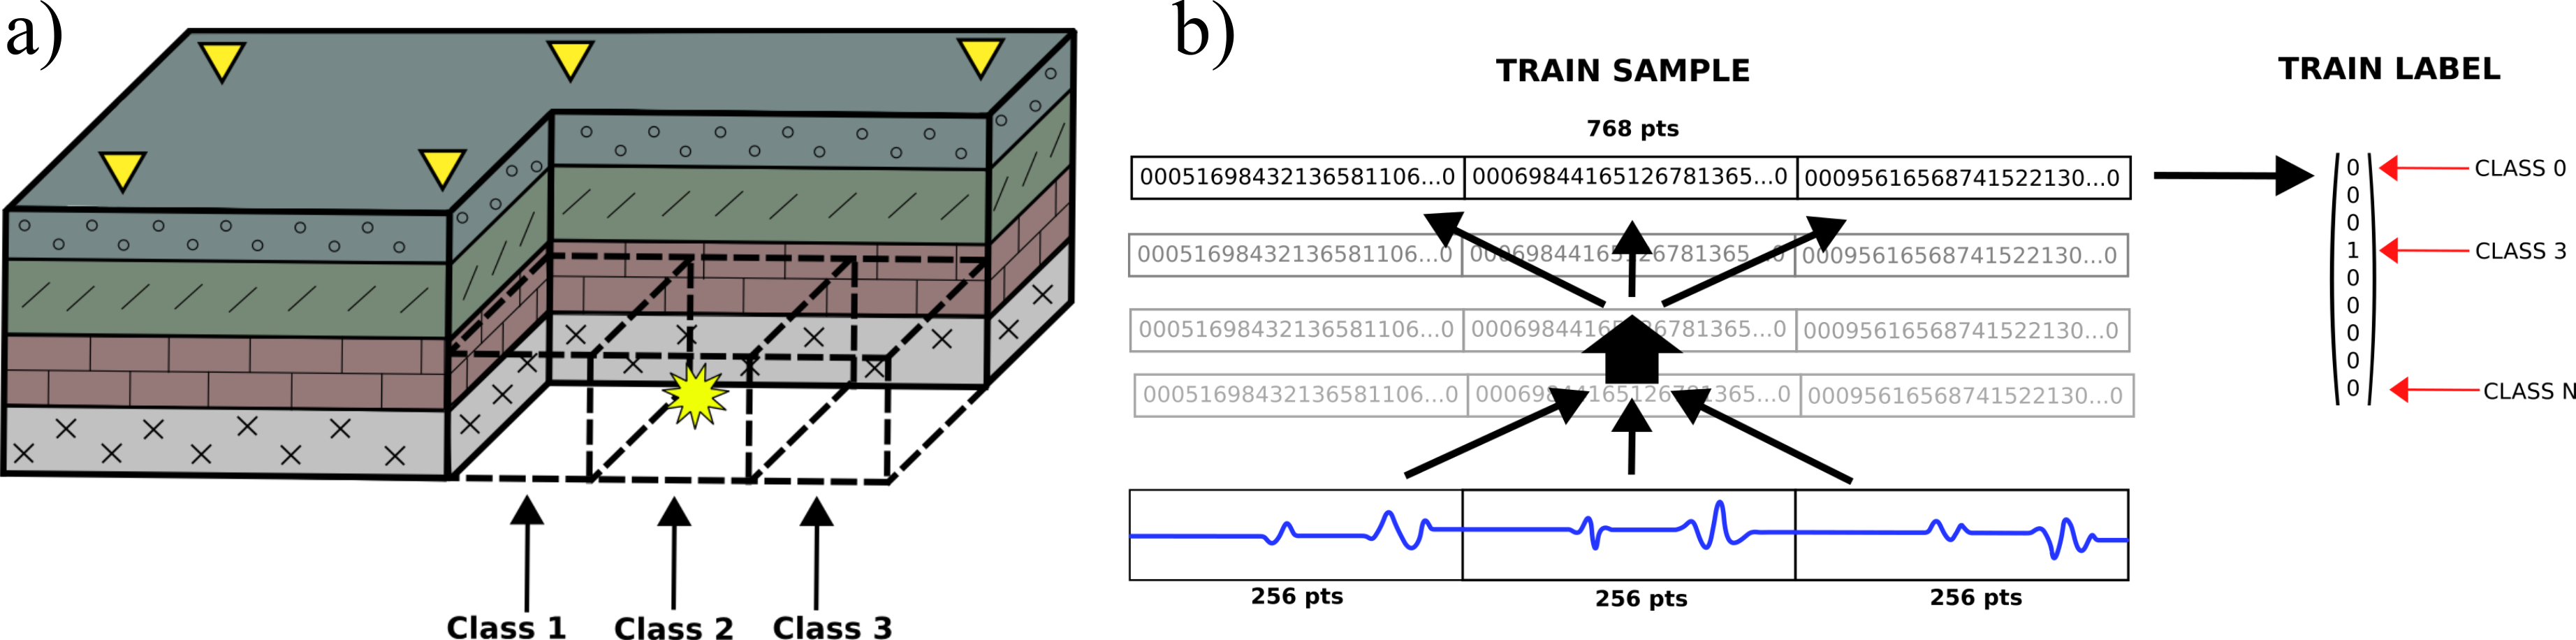
\includegraphics[width=0.85\linewidth,angle=0]{./AntonBiryukov_bibtex/classes.png}
\end{center}
\vspace{-4mm}
\caption{An illustration of the signal classification concept. The signals originating from the locations on the grid (a) are then transformed into a feature space and labeled by the class containing the event origin.}
\label{fig:classes}
\end{figure*}


It is valuable to compare the performance of different rather simple classifiers on this problem before moving towards a more complex solution. Therefore, a comparison of prediction accuracy was done between a non-generalizing algorithm (K-nearest-neighbors, \cite{}) and linear classifiers (logistic regression\cite{} and Support Vector Classifier \cite{}). The comparison can help choose the more robust classification method for the future work, as well as identify the generalization character of the problem. The picked classifiers are easy to tune since the parametrization is done through one or two parameters, and as such serve as great candidates for a preliminary analysis. 

Python-based Scikit-Learn package was chosen as an implementation of the aforementioned algorithms. The fine-tuning of the internal algorithm parameters, e.g. regularization parameter $C$ for logistic regression and SVC, has been done through exhaustive grid search over the parameter space. The purpose of fine-tuning is to find the optimal set of parameters producing the highest prediction accuracy on the test set.

The output results of the classification can be interpreted in several ways. Here we limit ourselves to the interpretation of the confusion matrix of the test set. The elements of the confusion matrix $c_{i,j}$ show the number of observations from class $i$ predicted into class $j$. As a result, non-zero off-diagonal elements indicate the number of mislabeled observations, whereas the diagonal elements indicate the number of correctly predicted observations.
\section{Results}
In this section we first demonstrate the estimated depth and origin location uncertainties as obtained from Monte - Carlo simulations, followed by the summary of classification accuracy using several different classifiers.
\subsection{Origin uncertainty estimation}
The origin depth uncertainty was estimated for the 1\% and 6\% velocity perturbation. For both simulations the true location of the event was $(X,Y,Z) = (4000,6000,3910)$, which corresponds to the location of the main shock of January 2015 Fox Creek swarm. The location centroids of Monte-Carlo simulated events for the two models are shown in Figure \ref{fig:sigma1} and Figure \ref{fig:sigma6}, respectively. One may see that in both cases the X and Y coordinates of the event are centered at their true values. The depth of the event is centered above the true focal depth in the case of 1\% model. In the 6\% model case the event depth shows a bi-modal distribution, with stronger mode centered above the depth. The weaker mode, however tends to center around the true depth of the event. The standard deviation of the depth shows a noticeable increase as the velocity perturbation increases.
\begin{figure*}[htb]
\begin{center}
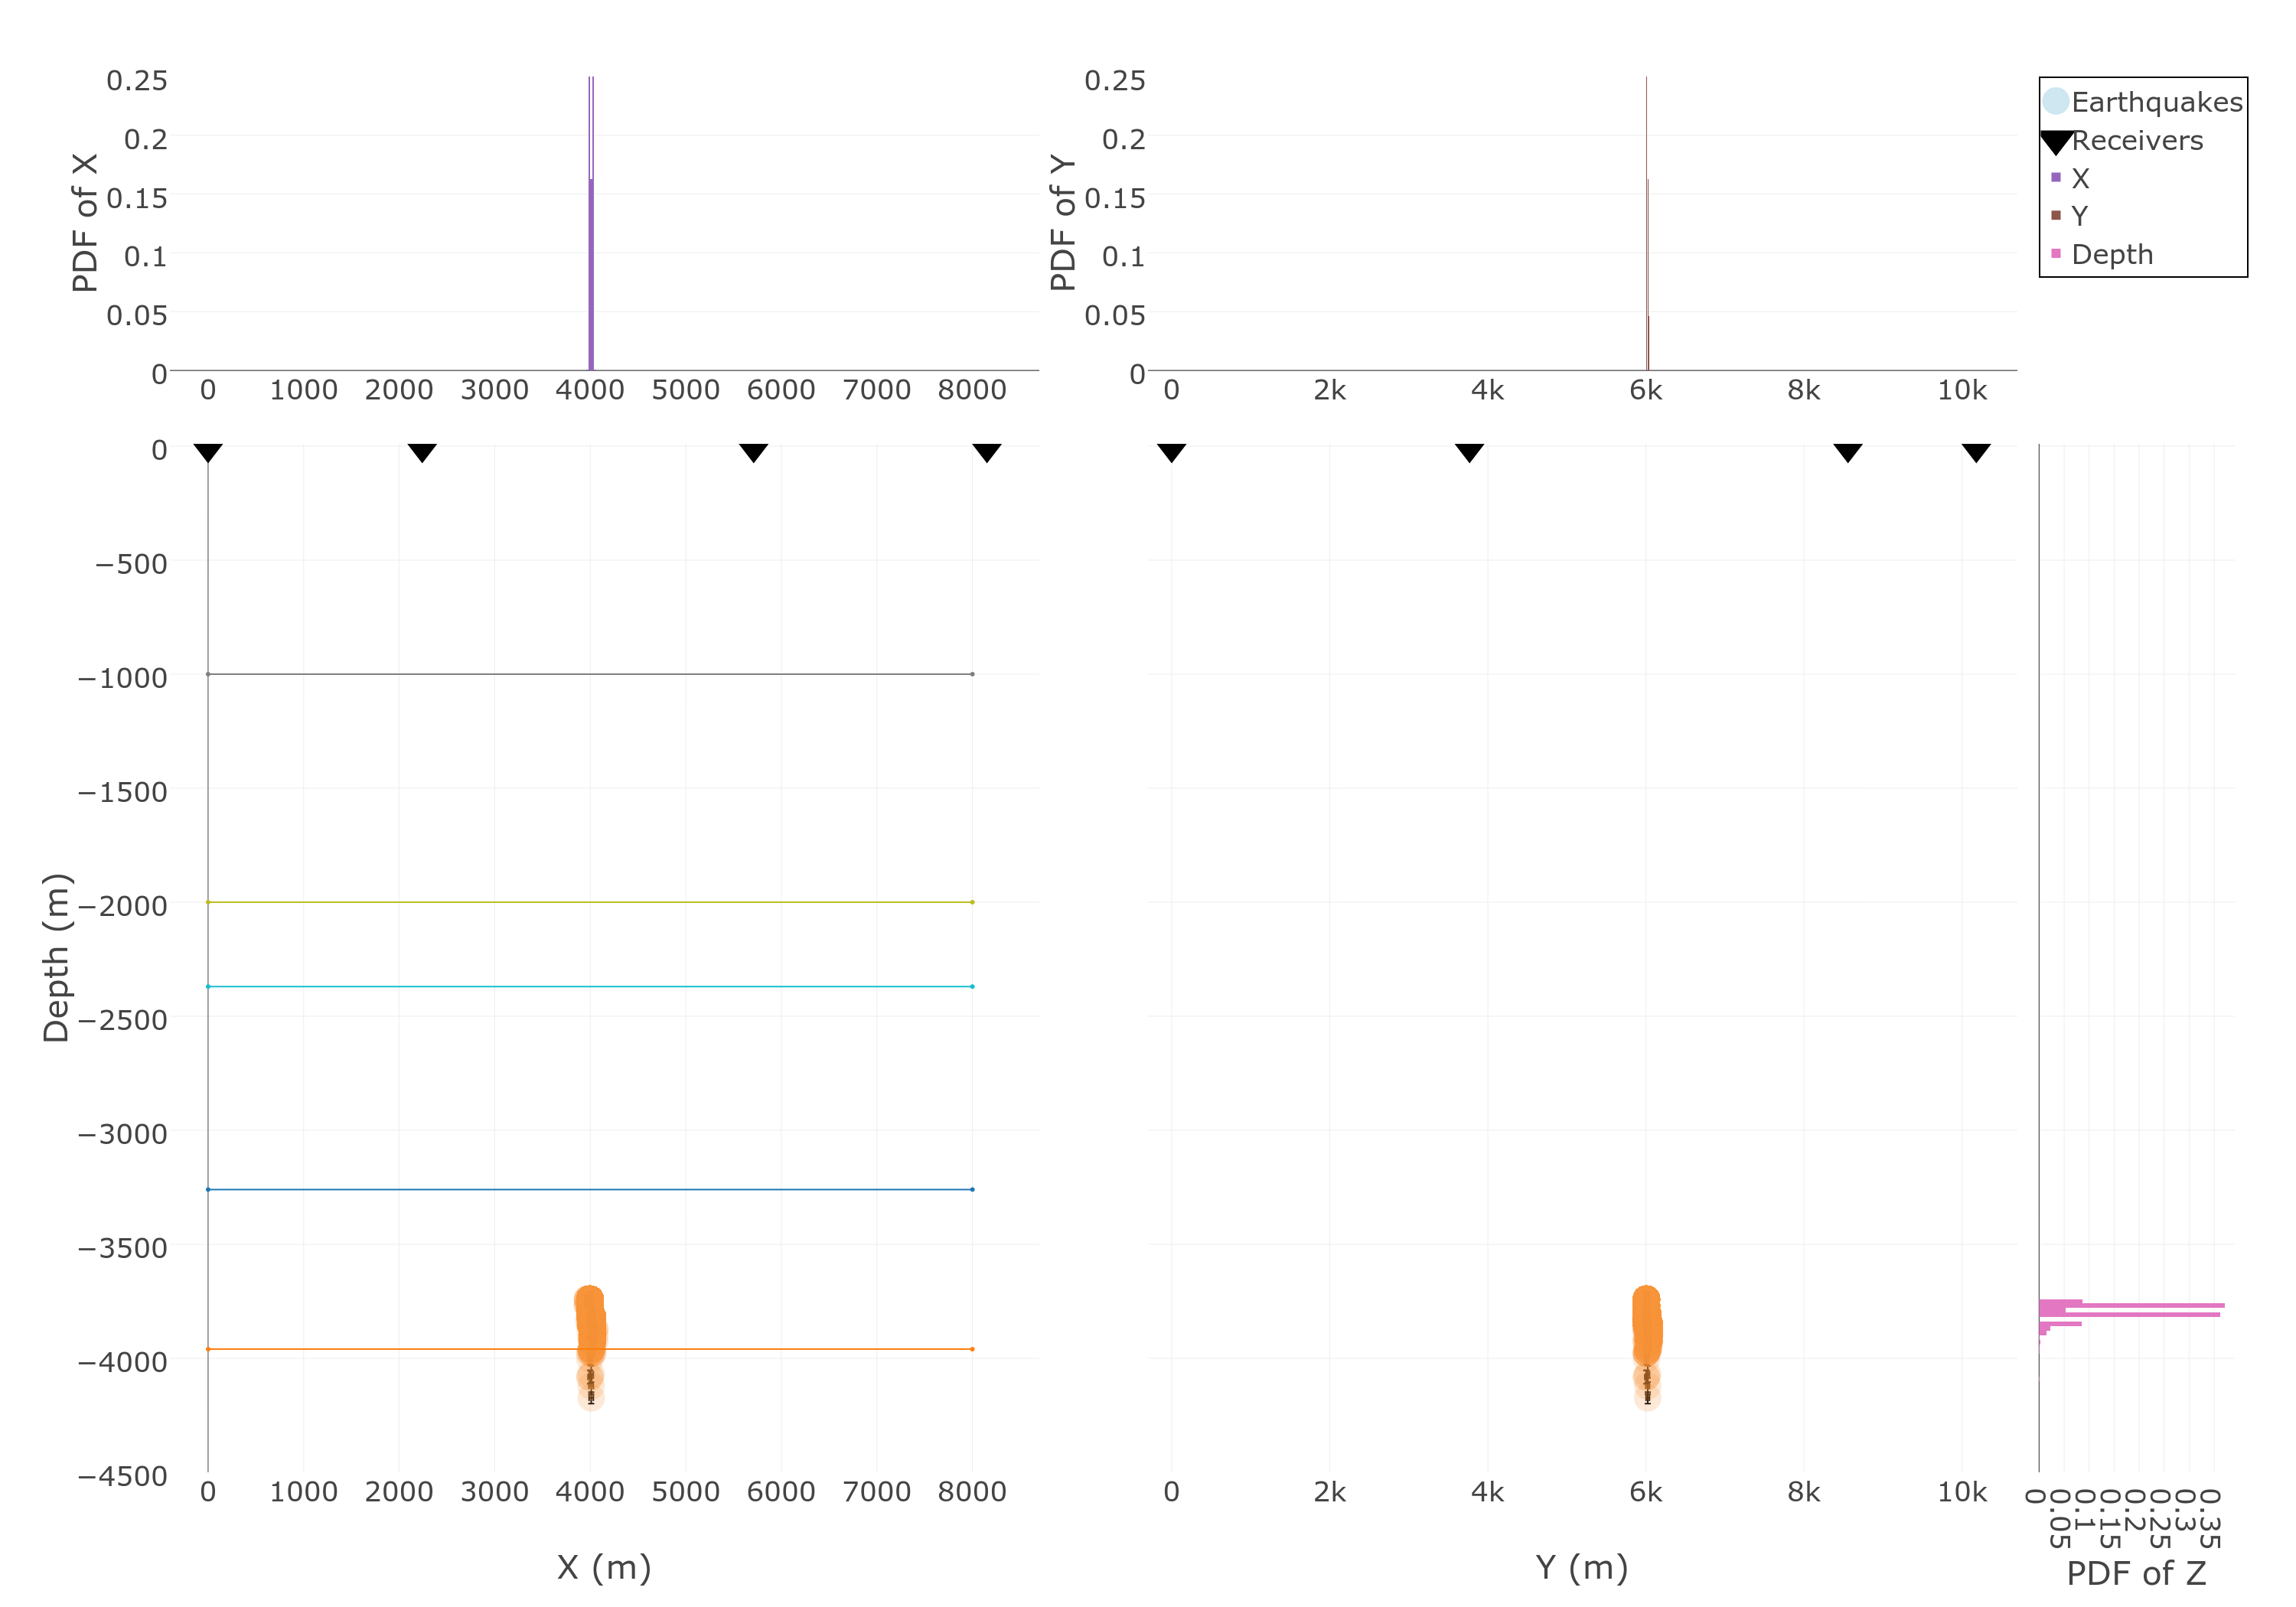
\includegraphics[width=0.85\linewidth,angle=0]{./AntonBiryukov_bibtex/Figure1_1pct.png}
\end{center}
\vspace{-4mm}
\caption{The results of the location of 1\% velocity perturbation Monte-Carlo simulated virtual events describing the true event at $(X,Y,Z) = (4000,6000,3910)$. The receivers are shown in black triangles, the virtual event centroids - in orange circles.}
\label{fig:sigma1}
\end{figure*}

\begin{figure*}[htb]
\begin{center}
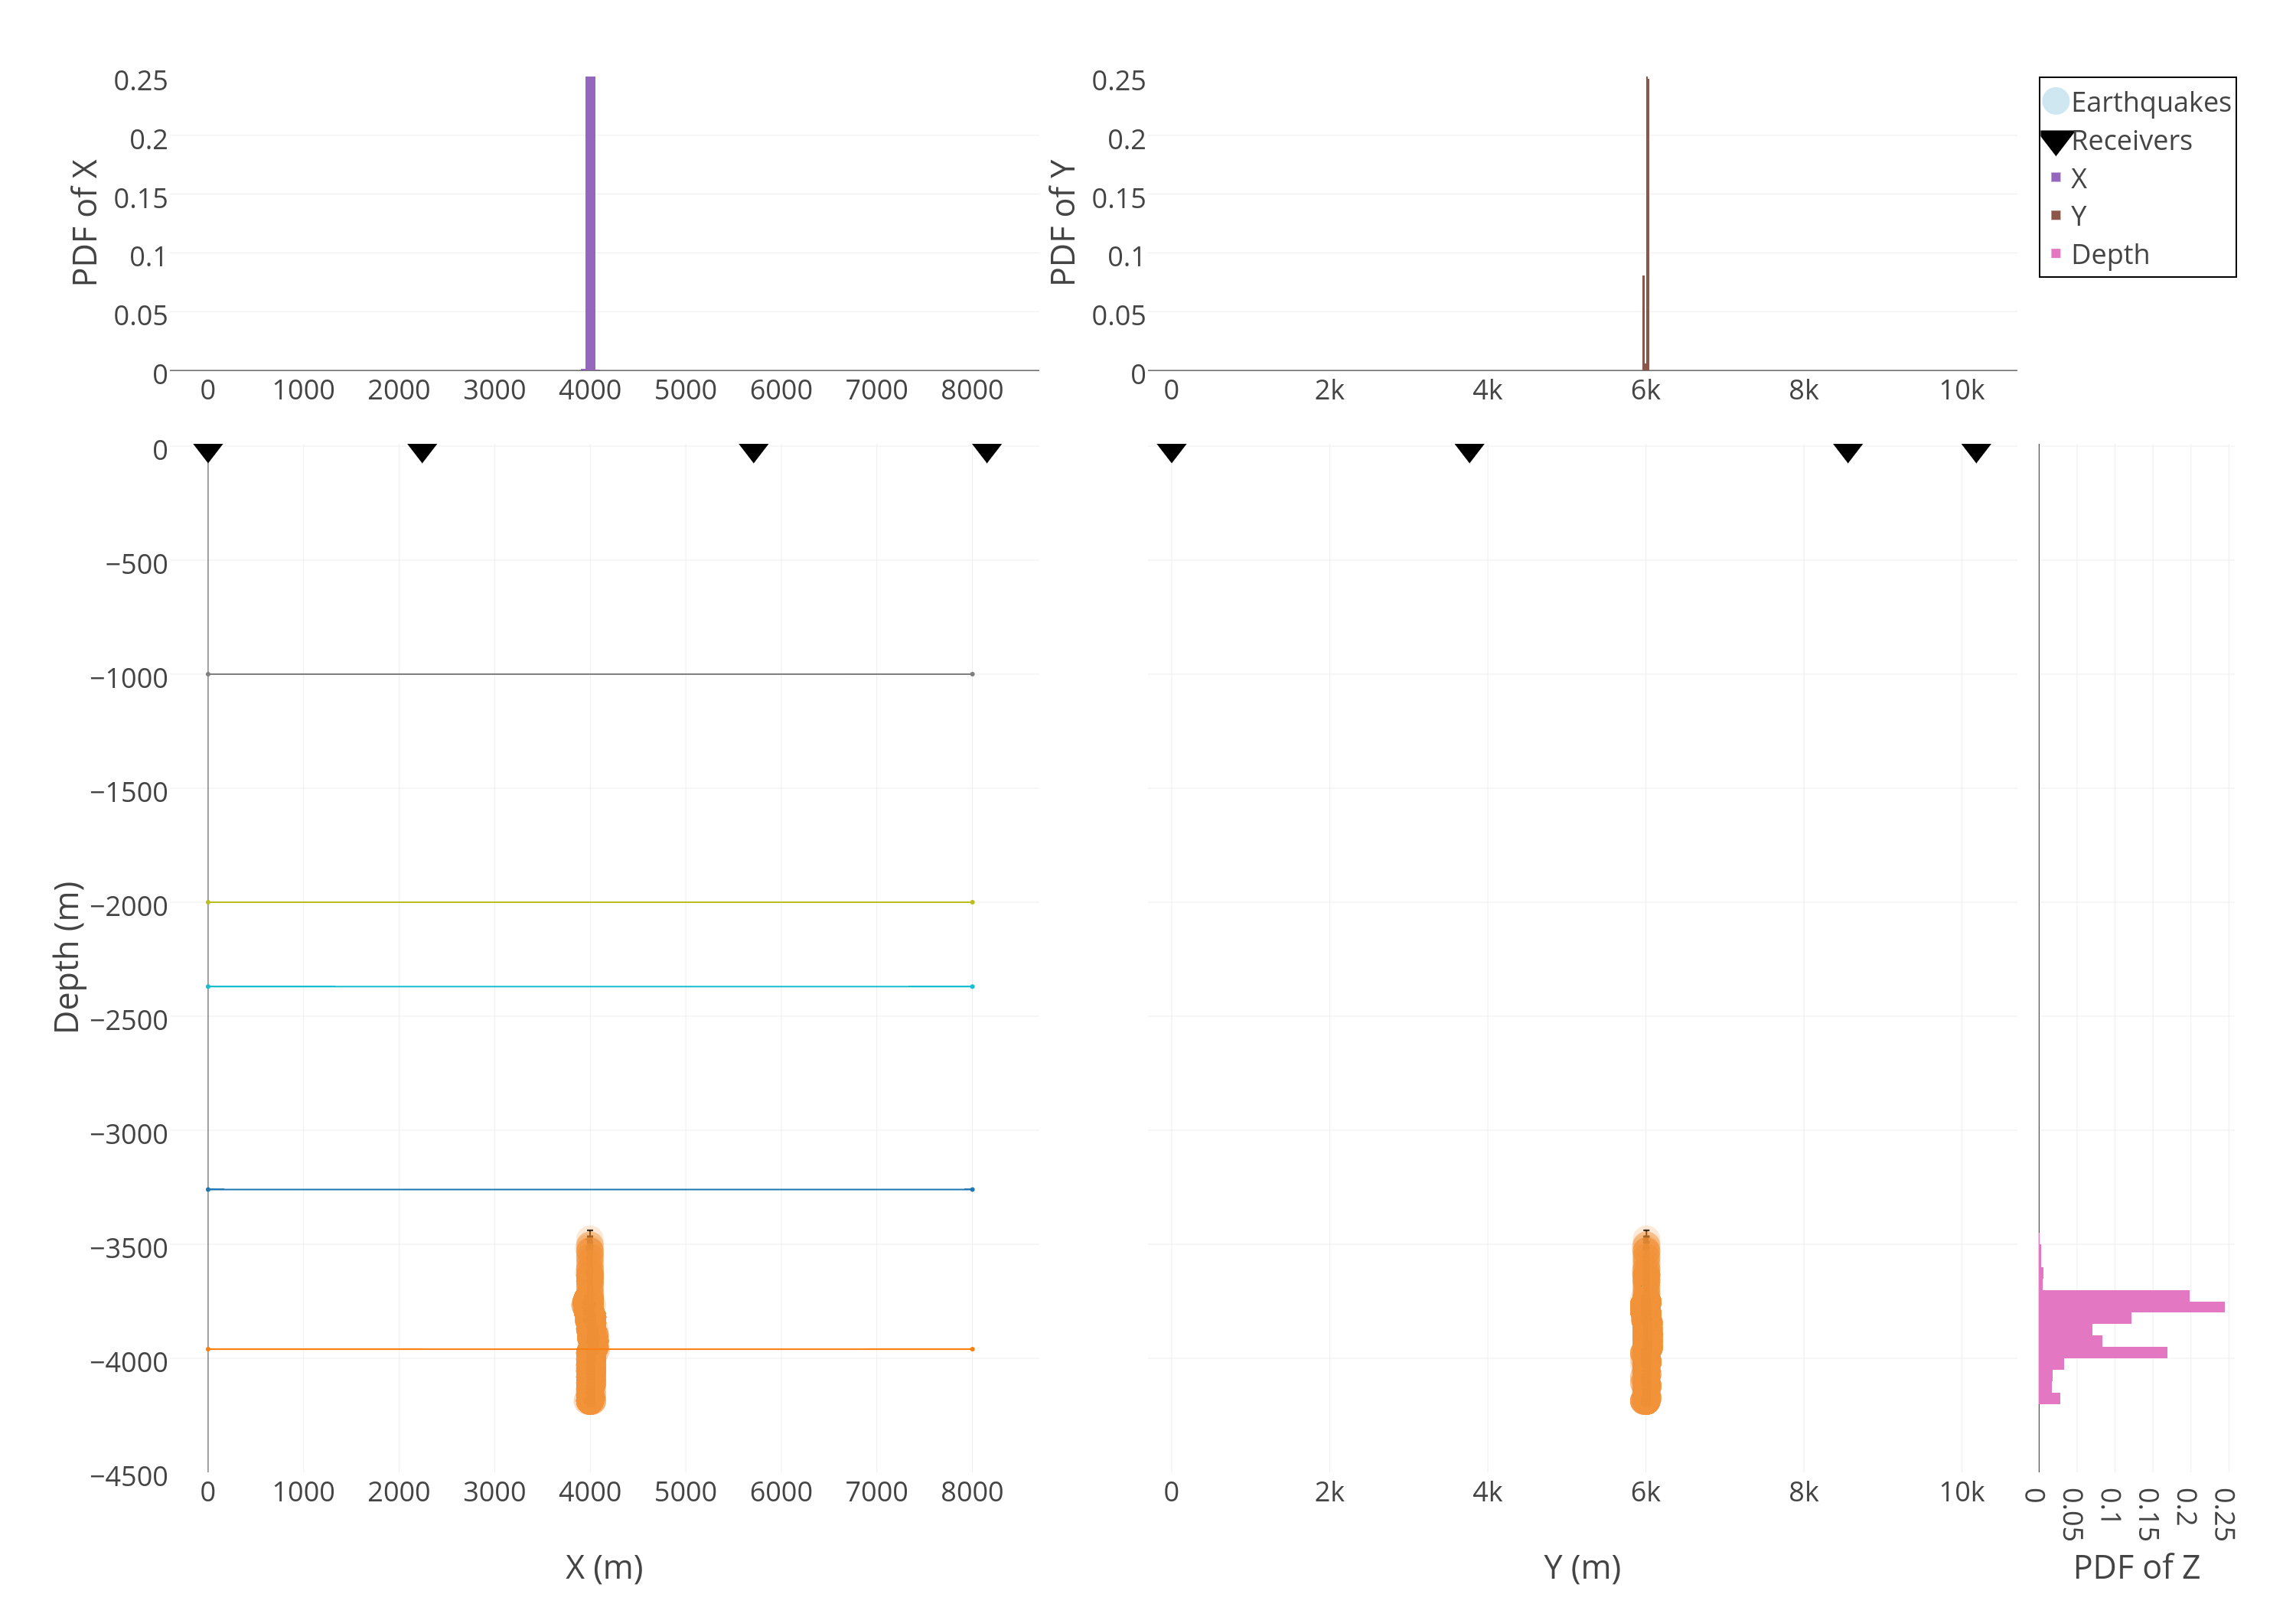
\includegraphics[width=0.85\linewidth,angle=0]{./AntonBiryukov_bibtex/Figure1_6pct.png}
\end{center}
\vspace{-4mm}
\caption{The results of the location of 6\% velocity perturbation Monte-Carlo simulated virtual events describing the true event at $(X,Y,Z) = (4000,6000,3910)$. The receivers are shown in black triangles, the virtual event centroids - in orange circles.}
\label{fig:sigma6}
\end{figure*}

For the sake of comparison, the origin errors for the individual locations due to the traveltime pick uncertainty of 10 ms are shown in Figure \ref{fig:ind_error}. One may notice that the uncertainties due to the picking error are an order of magnitude smaller than those shown previously in Figure \ref{fig:sigma1} and Figure \ref{fig:sigma6}.

\begin{figure}[htb]
\begin{center}
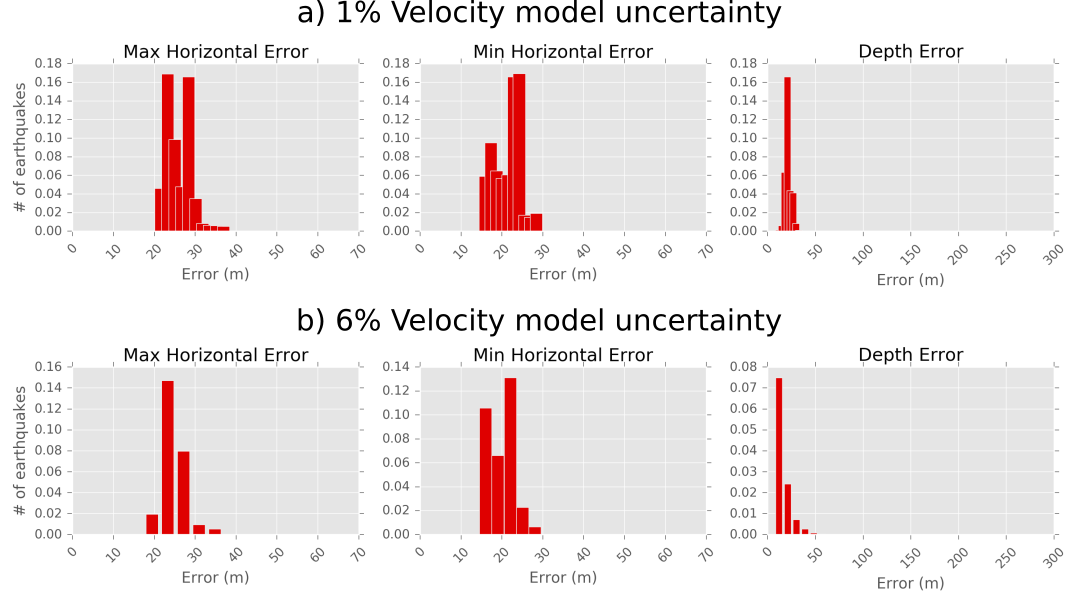
\includegraphics[width=0.85\linewidth,angle=0]{./AntonBiryukov_bibtex/figure_inderr.png}
\end{center}
\vspace{-4mm}
\caption{The distribution of the origin uncertainties for individual virtual event locations. The scale of the errors are an order of magnitude lower than the uncertainty due to the unknown velocity model}
\label{fig:ind_error}
\end{figure}

\subsection{Signal origin classification results}
The classification has been carried out on the database of 90 different earthquake origins distributed uniformly along the depth range of 2-5km and covering the area around the central Fox Creek seismicity cluster as shown in Figure \ref{fig:map_clusters}.
\begin{figure}[htb]
\begin{center}
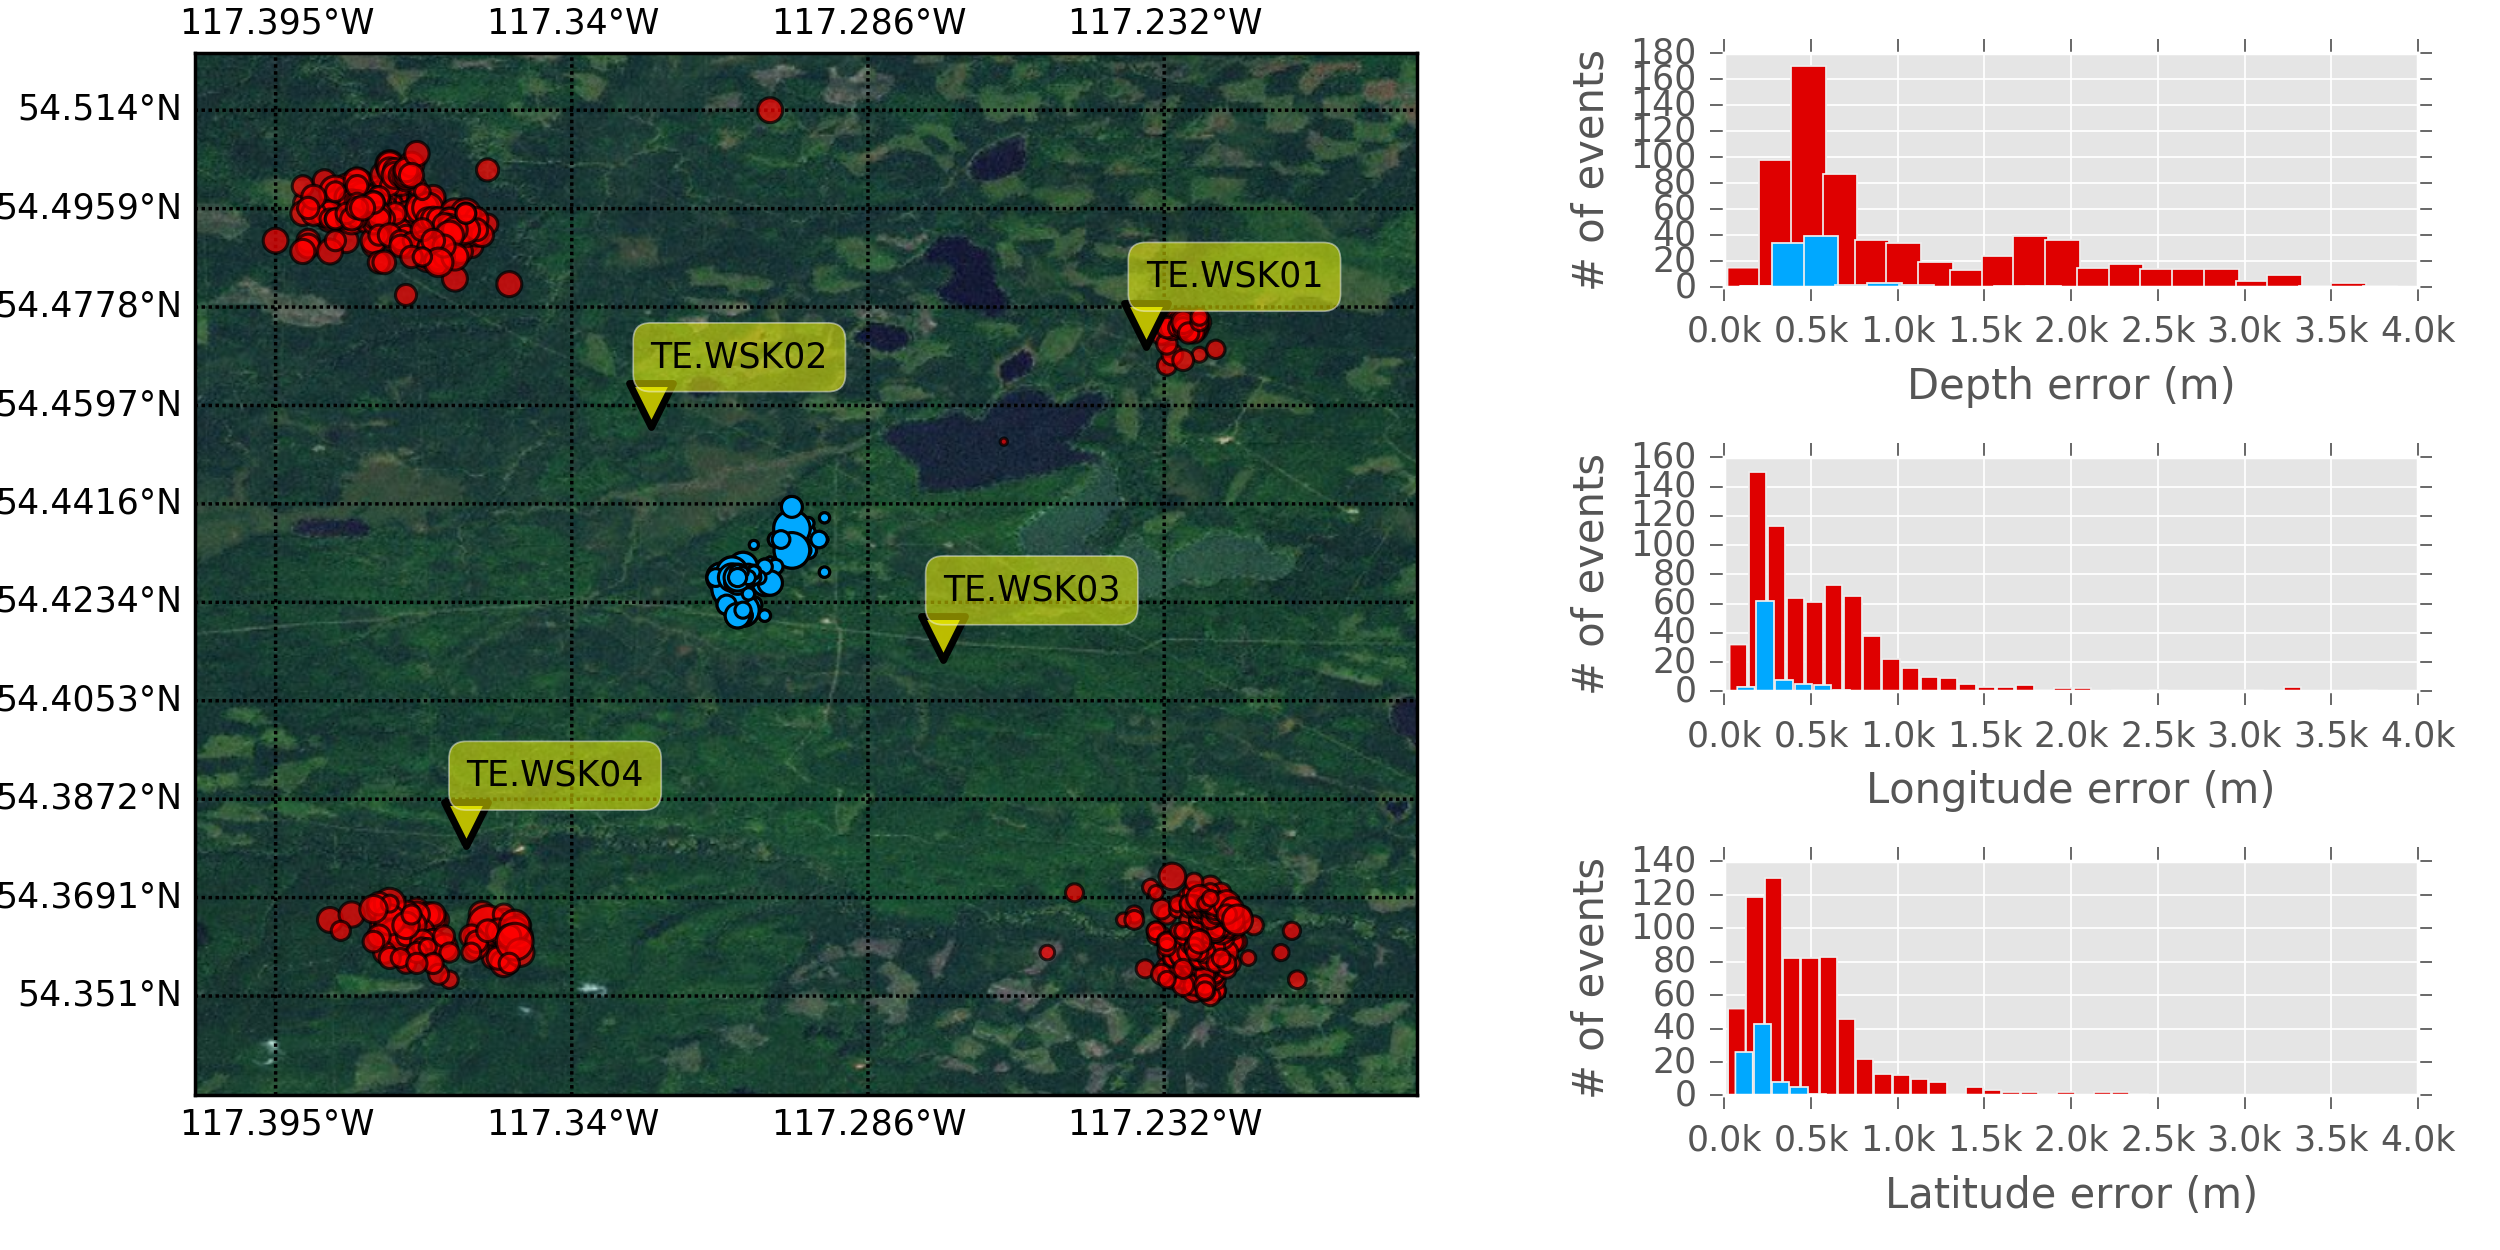
\includegraphics[width=0.85\linewidth,angle=0]{./AntonBiryukov_bibtex/figure_map_a.png}
\end{center}
\vspace{-4mm}
\caption{The distribution of induced seismicity in Fox Creek area for the events of winter 2015. The central cluster modeled in this study is shown in cyan.}
\label{fig:ind_error}
\end{figure}

Our main goal here was to demonstrate whether adding the signal features into the classification feature set produces a noticeable change in the 
The classification has been carried out for two feature sets: (i) 8 time arrival picks (2 per station and (ii) arrival picks combined with the signal features. T





\section{Discussion}
% TO DISCUSSION
Due to the location with respect to the array, the central cluster is characterized with lower values of horizontal location error compared to other clusters. However, as seen from the error distribution, the depth of the location is still poorly constrained for the central cluster and in some cases exceeds 500 m. Such an error is in reasonable agreement with the predicted depth error in the previous section.
\section{Conclusions}
PlaceHolder
%
We are using the cross reference package in this report, so if we want to refer to the convolutional model in (\ref{eq:your_name_convmodel}). In our text we call this equation by \verb"\ref{label}". 

\begin{equation}\label{eq:your_name_convmodel}
s(t) = w(t)\star r(t) + \eta(t).
\end{equation}

Did you know equations are part of sentences so you should use punctuation at the end of each equation?

The same happens referencing Figure \ref{fig:your_name_fig1}. (Use \verb"Figure \ref{label}"). 

If you want to say that \cite{VanderBaan2008a} did something then that's ok.
But maybe you prefer to put it as an statement \citep{VanderBaan2008a}?

\section{Use figures}

% Single Column figure!!!
\begin{figure}[htb]
\begin{center}
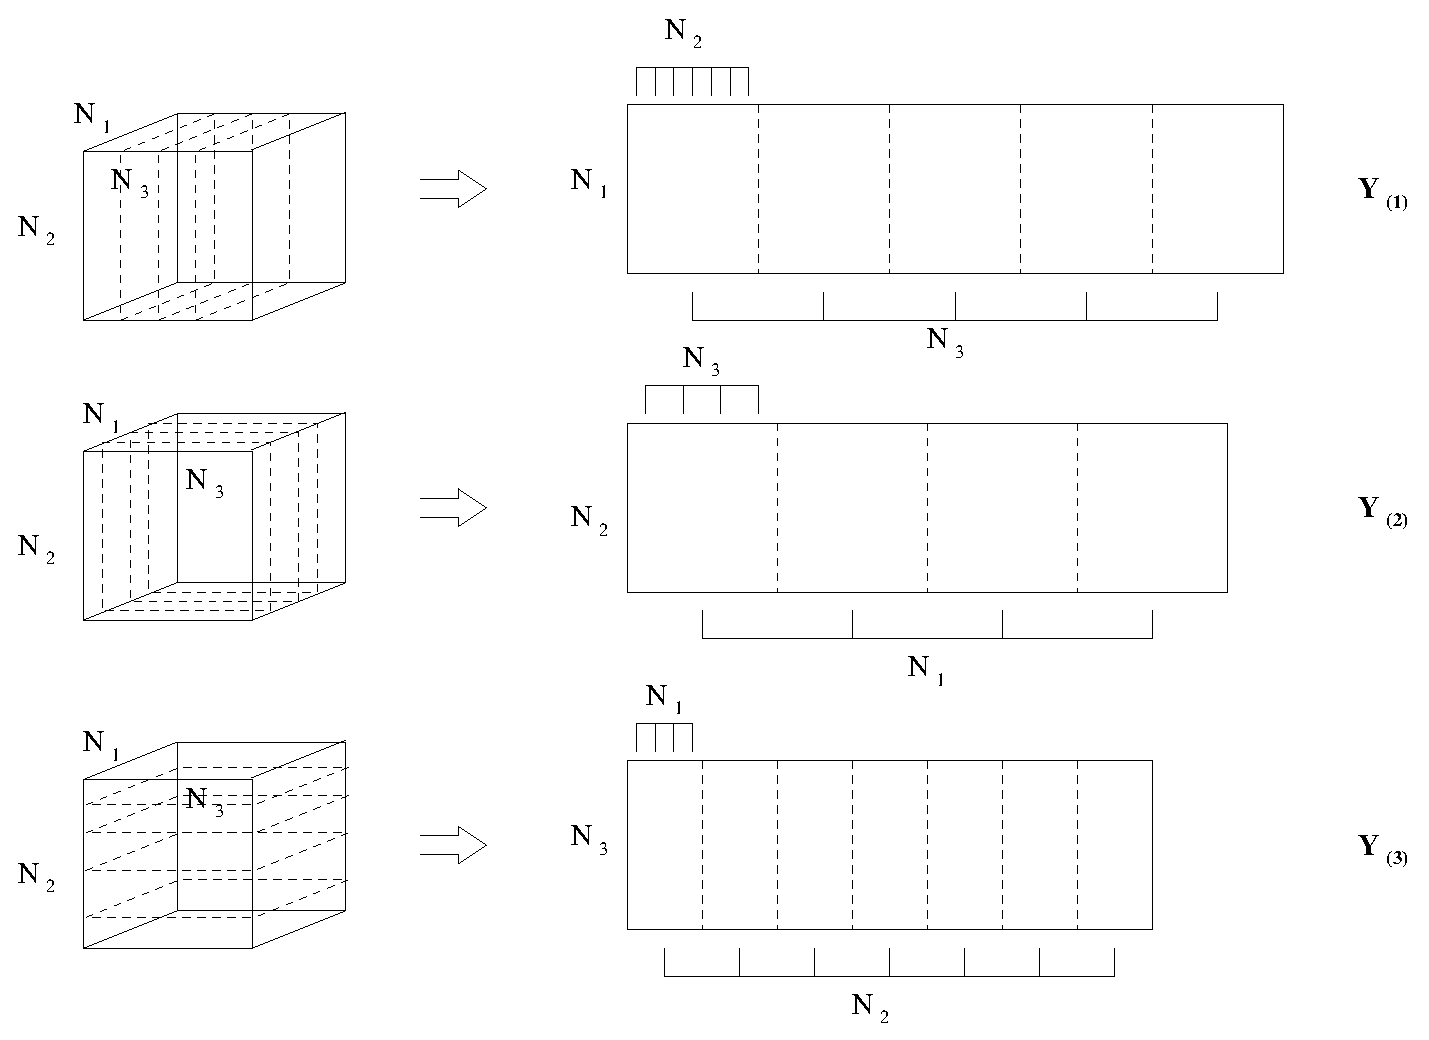
\includegraphics[width=0.7\linewidth,angle=0]{your_chapter_bibitem/fig1.eps}
\end{center}
\vspace{-4mm}
\caption{Your caption}
\label{fig:your_name_fig1}
\end{figure}
%

% Full page width figure!!!
\begin{figure*}[htb]
\begin{center}
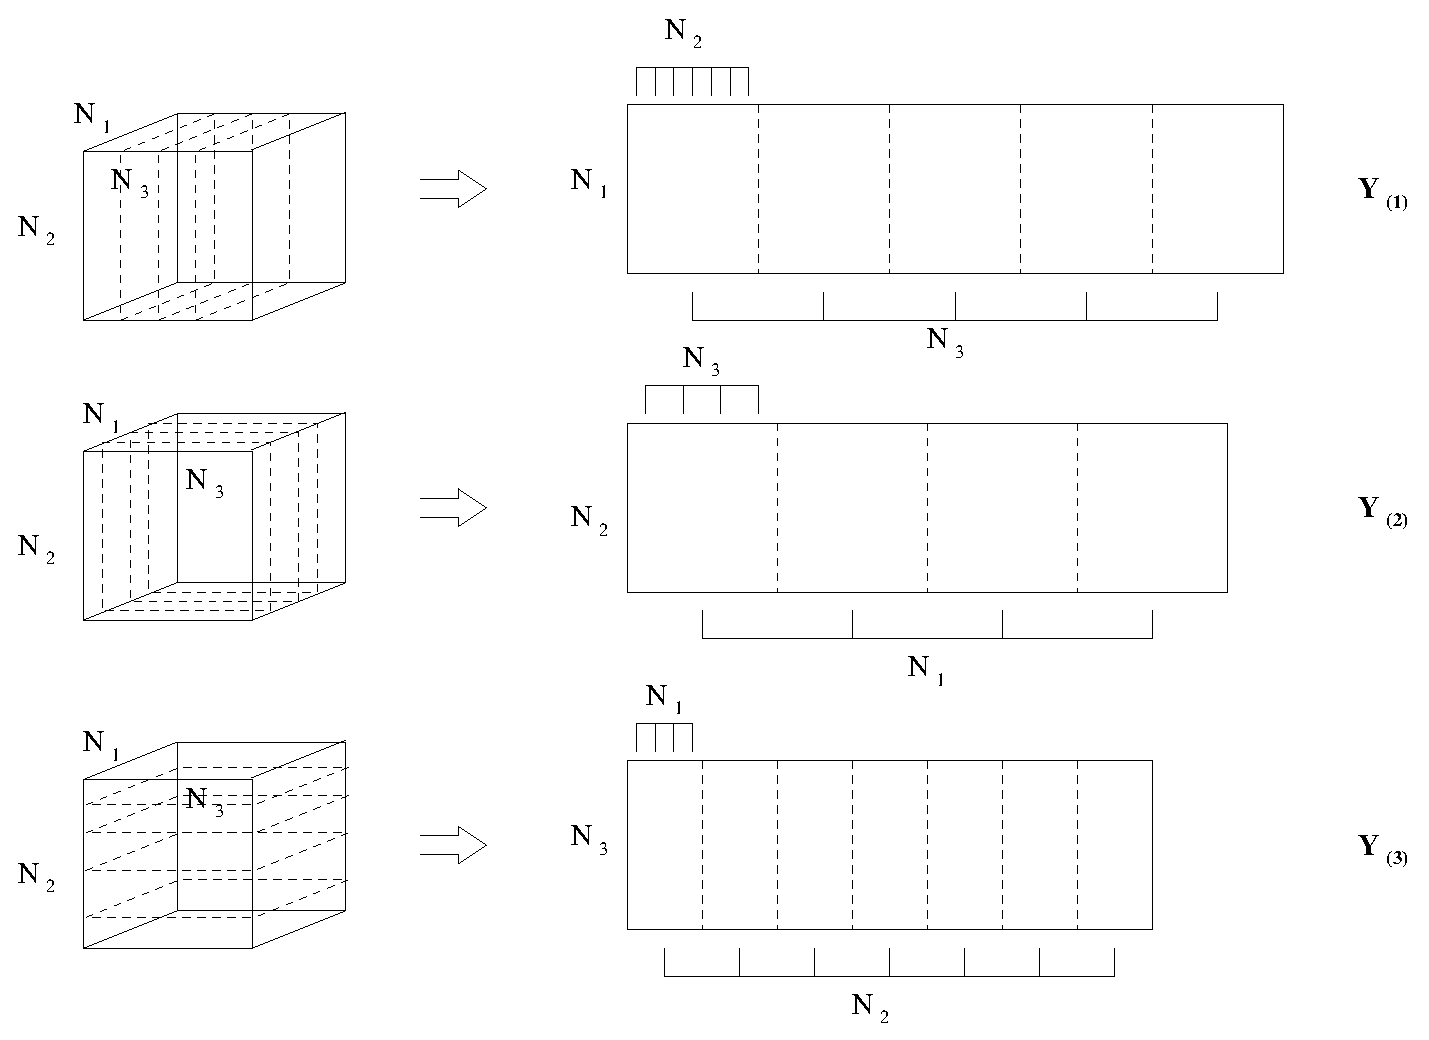
\includegraphics[width=0.7\linewidth,angle=0]{your_chapter_bibitem/fig1.eps}
\end{center}
\vspace{-4mm}
\caption{Your caption}
\label{fig:your_name_fig2}
\end{figure*}
%


%
\section{Acknowledgments}
%
The author would like to thank the sponsors of the Microseismic Industry Consortium for financial support.
%

% 
%\addcontentsline{toc}{section}{References}
\clearpage
\nocite{*}
\bibliographystyle{seg} 
\bibliography{AntonBiryukov_bibtex/example.bib}